\section*{8. Estimating the CDF and Statistical Functionals}\label{estimating-the-cdf-and-statistical-functionals}

\subsection*{8.1 Empirical distribution
function}\label{empirical-distribution-function}
The \textbf{empirical distribution function} \(\hat{F}_{n}\) is the CDF
that puts mass \(1/n\) at each data point \(X_{i}\). Formally,
\begin{align*}
\hat{F}_{n}(x) & = \frac{\sum_{i=1}^{n} I\left(X_{i} \leq x \right)}{n} \\
& = \frac{\#|\text{observations less than or equal to x}|}{n}
\end{align*}
where
\begin{align*}I\left(X_{i} \leq x\right) =
    \begin{cases}
      1   & \text{if } X_{i} \leq x \\
      0   & \text{if } X_{i} > x
    \end{cases}
\end{align*}

\textbf{Theorem 8.3}. At any fixed value of \(x\),
\begin{align*}\EXP\left( \hat{F}_{n}(x) \right) = F(x)
\quad\mathrm{and}\quad 
\VAR\left( \hat{F}_{n}(x) \right) = \frac{F(x)(1 - F(x))}{n}
\end{align*}
Thus,
\[
\MSE = \frac{F(x)(1 - F(x))}{n} \rightarrow 0
\]
and hence, \(\hat{F}_{n}(x) \xrightarrow{\textrm{P}} F(x)\).

\textbf{Theorem 8.4 (Glivenko-Cantelli Theorem)}. Let
\(X_{1}, \dots, X_{n} \sim F\). Then
\[
\sup _x |\hat{F}_{n}(x) - F(x)| \xrightarrow{\textrm{P}} 0
\]
(actually, \(\sup _x |\hat{F}_{n}(x) - F(x)|\) converges to 0 almost
surely.)

\subsection*{8.2 Statistical
Functionals}\label{statistical-functionals}
A \textbf{statistical functional} \(T(F)\) is any function of \(F\).
Examples are the mean \(\mu = \int x dF(x)\), the variance
\(\sigma^{2} = \int (x - \mu)^{2} dF(x)\) and the median
\(m = F^{-1}(1/2)\).
The \textbf{plug-in estimator} of \(\theta = T(F)\) is defined by
\[
\hat{\theta}_{n} = T(\hat{F}_{n})
\]
In other words, just plug in \(\hat{F}_{n}\) for the unknown \(F\).
A functional of the form \(\int r(x) dF(x)\) is called a \textbf{linear
functional}. Recall that \(\int r(x) dF(x)\) is defined to be
\(\int r(x) f(x) d(x)\) in the continuous case and
\(\sum_{j} r(x_{j}) f(x_{j})\) in the discrete.
The plug-in estimator for the linear functional
\(T(F) = \int r(x) dF(x)\) is:
\[
T(\hat{F}_{n}) = \int r(x) d\hat{F}_{n}(x) = \frac{1}{n} \sum_{i=1}^{n} r(X_{i})
\]
We have:
\[
T(\hat{F}_{n}) \approx N\left(T(F), \widehat{\SE}\right)
\]
An approximate \(1 - \alpha\) confidence interval for \(T(F)\) is then
\[
T(\hat{F}_{n}) \pm z_{\alpha/2} \widehat{\SE}
\]
We call this the \textbf{Normal-based interval}.

\subsection*{8.3 Technical Appendix}

\textbf{Theorem 8.12 (Dvoretsky-Kiefer-Wolfowitz (DKW) inequality)}. Let
\(X_{1}, \dots, X_{n}\) be iid from \(F\). Then, for any \(\epsilon > 0\),
\[
\PROB\left( \sup_x |F(x) - \hat{F}_{n}(x) | > \epsilon \right) \leq 2 e^{-2n\epsilon^{2}}
\]
From the DKW inequality, we can construct a confidence set. Let
\(\epsilon_{n}^{2} = \log(2/\alpha) / (2n)\),
\(L(x) = \max \{ \hat{F}_{n}(x) - \epsilon_{n}, \; 0 \}\) and
\(U(x) = \min \{\hat{F}_{n}(x) + \epsilon_{n}, 1 \}\). It follows that for
any \(F\),
\[
\PROB(F \in C_{n}) \geq 1 - \alpha
\]
To summarize: A \(1 - \alpha\) nonparametric confidence band for \(F\) is \((L(x), \; U(x))\) where
\begin{align*}
L(x) &= \max \{ \hat{F}_{n}(x) - \epsilon_{n}, \; 0 \} \\
U(x) &= \min \{ \hat{F}_{n}(x) + \epsilon_{n}, \; 1 \} \\
\epsilon_{n} &= \sqrt{\frac{1}{2n} \log \left( \frac{2}{\alpha} \right) }
\end{align*}

\subsection*{8.5 Exercises}

\textbf{Exercise 8.5.1}. Prove Theorem 8.3.

\textbf{Solution}. We have:
\[
\hat{F}_{n}(x) = \frac{\sum_{i=1}^{n} I\left(X_{i} \leq x \right)}{n}
\]
where
\begin{align*}I\left(X_{i} \leq x\right) =
    \begin{cases}
      1   & \text{if } X_{i} \leq x \\
      0   & \text{if } X_{i} > x
    \end{cases}       
\end{align*}
Thus,
\begin{align*}
\EXP(\hat{F}_{n}(x)) & = n^{-1} \sum_{i = 1}^{n} \EXP(I\left(X_{i} \leq x \right)) \\
 & = n^{-1} \sum_{i = 1}^{n} \PROB\left(X_{i} \leq x \right) \\
 & = n^{-1} \sum_{i = 1}^{n} F(x) \\
 & = F(x)
\end{align*}
\begin{align*}
\EXP(\hat{F}_{n}(x)^{2}) & = n^{-2} \EXP \left( \sum_{i = 1}^{n} I\left(X_{i} \leq x \right) \right)^{2} \\
& = n^{-2} \EXP \left( \sum_{i = 1}^{n} I\left(X_{i} \leq x \right)^{2} 
+ \sum_{i = 1}^{n} \sum_{j = 1, j \neq i}^{n} I\left(X_{i} \leq x \right) I\left(X_{j} \leq x \right) \right) \\
& = n^{-2} \left( \sum_{i = 1}^{n} \EXP \left( I\left(X_{i} \leq x \right)^{2} \right)
+ \sum_{i = 1}^{n} \sum_{j = 1, j \neq i}^{n} \EXP \left( I\left(X_{i} \leq x \right) I\left(X_{j} \leq x \right) \right) \right) \\
& = n^{-2} \left( \sum_{i = 1}^{n} \EXP \left( I\left(X_{i} \leq x \right) \right)
+ \sum_{i = 1}^{n} \sum_{j = 1, j \neq i}^{n} \EXP \left( I\left(X_{i} \leq x \right) \right) \EXP \left( I\left(X_{j} \leq x \right) \right) \right) \\
& = n^{-2} \left( \sum_{i = 1}^{n} \PROB\left(X_{i} \leq x \right) 
+ \sum_{i = 1}^{n} \sum_{j = 1, j \neq i}^{n} \PROB\left(X_{i} \leq x \right) \PROB\left(X_{j} \leq x \right)  \right) \\
&= n^{-2} \left( \sum_{i = 1}^{n} F(x)
+ \sum_{i = 1}^{n} \sum_{j = 1, j \neq i}^{n} F(x)^{2}  \right) \\
&= n^{-2} \left( nF(x) + (n^{2} - n)F(x)^{2} \right) \\
&= n^{-1} ( F(x) + (n - 1) F(x)^{2} )
\end{align*}
Therefore,
\[
\VAR(\hat{F}_{n}(x)) 
= \EXP(\hat{F}_{n}(x)^{2}) - \EXP(\hat{F}_{n}(x))^{2}
= F(x) /n + (1 - 1/n)F(x)^{2} - F(x)^{2}
= \frac{F(x)(1 - F(x))}{n}
\]
Finally,
\[
\MSE = (\text{bias}(F(x)))^{2} + \VAR(F(x)) = (\EXP(\hat{F}_{n}(x)) - F(x))^{2} + \VAR(F(x)) = \VAR(F(x)) = \frac{F(x)(1 - F(x))}{n} \rightarrow 0
\]

\textbf{Exercise 8.5.2}. Let
\(X_{1}, \dots, X_{n} \sim \text{Bernoulli}(p)\) and let
\(Y_{1}, \dots, Y_m \sim \text{Bernoulli}(q)\).
\begin{itemize}[tightlist]
\item
  Find the plug-in estimator and estimated standard error for \(p\).
\item
  Find an approximate 90-percent confidence interval for \(p\).
\item
  Find the plug-in estimator and estimated standard error for \(p - q\).
\item
  Find an approximate 90-percent confidence interval for \(p - q\).
\end{itemize}

\textbf{Solution}.
\textbf{(a)}
\(p\) is the mean of \(\text{Bernoulli}(p)\), so its plugin estimator is
\(\hat{p} = \EXP(\hat{F}_{n}) = n^{-1} \sum_{i=1}^{n} X_{i}  = \bar{X}_{n}\).
\(\sqrt{p(1-p)}\) is the standard deviation of \(\text{Bernoulli}(p)\),
so the plugin estimator for the standard error is
\(\sqrt{\frac{\hat{p}(1-\hat{p})}{n}} = \sqrt{\frac{\bar{X}_{n}(1 - \bar{X}_{n})}{n}}\).
\textbf{(b)}
The 90-percent confidence interval for \(p\) is
\(\hat{p} \pm z_{0.05} \hat{se}(\hat{p})= \bar{X}_{n} \pm z_{0.05} \sqrt{\frac{\bar{X}_{n}(1-\bar{X}_{n})}{n}}\).
\textbf{(c)}
The plug-in estimator for \(\theta = p - q\) is
\(\hat{\theta} = \hat{p} - \hat{q} = \bar{X}_{n} - \bar{Y}_m\).
The standard error of \(\hat{\theta}\) is
\[
\SE = \sqrt{\VAR(\hat{p} - \hat{q})} = \sqrt{\VAR(\hat{p}) + \VAR(\hat{q})} = \sqrt{\frac{\hat{p}(1 - \hat{p})}{n} + \frac{\hat{q}(1 - \hat{q})}{n}} = \sqrt{\frac{\bar{X}_{n}(1 - \bar{X}_{n})}{n} + \frac{\bar{Y}_m(1 - \bar{Y}_m)}{n}} 
\]
\textbf{(d)}
The 90-percent confidence interval for \(\theta = p - q\) is
\[
\hat{\theta} \pm z_{0.05} \hat{se}(\hat{\theta}) 
= \bar{X}_{n} -
\bar{Y}m \pm z_{0.05}
\sqrt{\frac{\bar{X}_{n}(1 - \bar{X}_{n})}{n} + \frac{\bar{Y}_m(1 - \bar{Y}_m)}{n}}
\]

\textbf{Exercise 8.5.3}. (Computer Experiment) Generate 100 observations
from a \(N(0, 1)\) distribution. Compute a 95 percent confidence band
for the CDF \(F\). Repeat this 1000 times and see how often the
confidence band contains the true function. Repeat using data from a
Cauchy distribution.

\begin{python}
import math
import numpy as np
import pandas as pd
from scipy.stats import norm, cauchy
import matplotlib.pyplot as plt
from tqdm import tqdm
\end{python}

\begin{python}
# One iteration wtih Normal distribution
n = 100
alpha = 0.05
r = norm.rvs(size=n)
epsilon = math.sqrt((1 / (2 * n)) * math.log(2 / alpha))
F_n = lambda x : sum(r < x) / n
L_n = lambda x : max(F_n(x) - epsilon, 0)
U_n = lambda x : min(F_n(x) + epsilon, 1)
xx = sorted(r)
df = pd.DataFrame({
    'x': xx, 
    'F_n': np.array(list(map(F_n, xx))), 
    'U_n': np.array(list(map(U_n, xx))), 
    'L_n': np.array(list(map(L_n, xx))), 
    'CDF': np.array(list(map(norm.cdf, xx)))
})
df['in_bounds'] = (df['U_n'] >= df['CDF']) & (df['CDF'] >= df['L_n'])
plt.plot( 'x', 'L_n', data=df, color='red')
plt.plot( 'x', 'U_n', data=df, color='green')
plt.plot( 'x', 'CDF', data=df, color='purple')
plt.legend()
\end{python}

\begin{figure}[H]
\centering
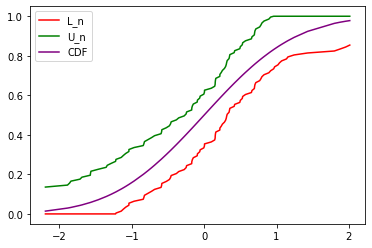
\includegraphics{Figure-08-01}
\end{figure}

    

\begin{python}
# 1000 iterations with Normal distribution
bounds = []
for k in tqdm(range(1000)):
    n = 100
    alpha = 0.05
    r = norm.rvs(size=n)
    epsilon = math.sqrt((1 / (2 * n)) * math.log(2 / alpha))
    F_n = lambda x : sum(r < x) / n
    L_n = lambda x : max(F_n(x) - epsilon, 0)
    U_n = lambda x : min(F_n(x) + epsilon, 1)
    # xx = sorted(r)
    xx = r # No need to sort without plotting
    
    df = pd.DataFrame({
        'x': xx, 
        'F_n': np.array(list(map(F_n, xx))), 
        'U_n': np.array(list(map(U_n, xx))), 
        'L_n': np.array(list(map(L_n, xx))), 
        'CDF': np.array(list(map(norm.cdf, xx)))
    })
    all_in_bounds = ((df['U_n'] >= df['CDF']) & (df['CDF'] >= df['L_n'])).all()
    bounds.append(all_in_bounds)
    
print('Average fraction in bounds: %.3f' % np.array(bounds).mean())
\end{python}
\begin{console}
100\%|███████████████████████████████████████████████████████████████████████████
████████████████████████████████████████████████████████████████████████████████
████████████████████████████████████████| 1000/1000 [01:05<00:00, 15.19it/s]
\end{console}
\begin{console}
Average fraction in bounds: 0.954
\end{console}

\begin{python}
# One iteration wtih Cauchy distribution
n = 100
alpha = 0.05
r = cauchy.rvs(size=n)
epsilon = math.sqrt((1 / (2 * n)) * math.log(2 / alpha))
F_n = lambda x : sum(r < x) / n
L_n = lambda x : max(F_n(x) - epsilon, 0)
U_n = lambda x : min(F_n(x) + epsilon, 1)
xx = sorted(r)
df = pd.DataFrame({
    'x': xx, 
    'F_n': np.array(list(map(F_n, xx))), 
    'U_n': np.array(list(map(U_n, xx))), 
    'L_n': np.array(list(map(L_n, xx))), 
    'CDF': np.array(list(map(norm.cdf, xx)))
})
df['in_bounds'] = (df['U_n'] >= df['CDF']) & (df['CDF'] >= df['L_n'])
plt.plot( 'x', 'L_n', data=df, color='red')
plt.plot( 'x', 'U_n', data=df, color='green')
plt.plot( 'x', 'CDF', data=df, color='purple')
plt.legend()
\end{python}

\begin{figure}[H]
\centering
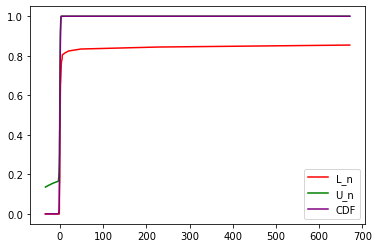
\includegraphics{Figure-08-02}
\end{figure}


\begin{python}
# 1000 iterations with Cauchy distribution
bounds = []
for k in tqdm(range(1000)):
    n = 100
    alpha = 0.05
    r = cauchy.rvs(size=n)
    epsilon = math.sqrt((1 / (2 * n)) * math.log(2 / alpha))
    F_n = lambda x : sum(r < x) / n
    L_n = lambda x : max(F_n(x) - epsilon, 0)
    U_n = lambda x : min(F_n(x) + epsilon, 1)
    # xx = sorted(r)
    xx = r # No need to sort without plotting
    df = pd.DataFrame({
        'x': xx, 
        'F_n': np.array(list(map(F_n, xx))), 
        'U_n': np.array(list(map(U_n, xx))), 
        'L_n': np.array(list(map(L_n, xx))), 
        'CDF': np.array(list(map(norm.cdf, xx)))
    })
    all_in_bounds = ((df['U_n'] >= df['CDF']) & (df['CDF'] >= df['L_n'])).all()
    bounds.append(all_in_bounds)
    
print('Average fraction in bounds: %.3f' % np.array(bounds).mean())
\end{python}
\begin{console}
100\%|███████████████████████████████████████████████████████████████████████████
████████████████████████████████████████████████████████████████████████████████
████████████████████████████████████████| 1000/1000 [01:04<00:00, 15.42it/s]
\end{console}
\begin{console}
Average fraction in bounds: 0.209
\end{console}

\textbf{Exercise 8.5.4}. Let \(X_{1}, \dots, X_{n} \sim F\) and let
\(\hat{F}_{n}(x)\) be the empirical distribution function. For a fixed
\(x\), use the central limit Theorem to find the limiting distribution
of \(\hat{F}_{n}(x)\).

\textbf{Solution}.
We have:
\[
\hat{F}_{n}(x) = \frac{\sum_{i=1}^{n} I\left(X_{i} \leq x \right)}{n}
\]
where
\begin{align*}I\left(X_{i} \leq x\right) =
    \begin{cases}
      1   & \text{if } X_{i} \leq x \\
      0   & \text{if } X_{i} > x
    \end{cases}       
\end{align*}
Let \(Y_{i} = I\left(X_{i} \leq x \right)\) for some fixed \(x\). From the
central limit Theorem,
\begin{align*}
\sqrt{n} (\bar{Y}_{n} - \mu_Y) & \leadsto N(0, \sigma_Y^{2}) \\
\bar{Y}_{n} & \leadsto N(\mu_Y, \sigma_Y^{2} / n)
\end{align*}
We can estimate the mean \(\mu_Y\) as
\[
\EXP(\hat{\mu}_{Y}) = \EXP(\bar{Y}_{n}) = n^{-1} \sum_{i=1}^{n} \EXP(I(X_{i} \leq x)) = n^{-1} \sum_{i=1}^{n} F(x) = \hat{F}_{n}(x).
\]
We can estimate the variance \(\sigma_Y^{2}\) as
\begin{align*}
\EXP(\hat{\sigma}_{Y}^{2}) 
  = \EXP(\VAR(\bar{Y}_{n})) 
& = n^{-1} \sum_{i=1}^{n} \EXP((Y_{i} - \bar{Y}_{n})^{2}) 
\\
& = n^{-1} \sum_{i=1}^{n} \left( \EXP(Y_{i}^{2}) - 2 \EXP(Y_{i} \bar{Y}_{n}) + \EXP(\bar{Y}_{n}^{2}) \right) 
\\
& \leq n^{-1} \sum_{i=1}^{n} \left( \EXP(Y_{i}) + \EXP(\bar{Y}_{n}^{2}) \right) \leq 2
\end{align*}
Therefore, for large \(n\), the limiting distribution has variance that
goes to 0 -- so \(\bar{Y}_{n} \leadsto \mu_Y\), or
\(I\left(X_{i} \leq x \right) \leadsto F(x)\) for every x. Then,
\(\hat{F}_{n}(x) \leadsto n^{-1} \sum_{i=1}^{n} F(x) = F(x)\),
and, as expected, \(F\) is the limiting distribution of \(F_n\).

\textbf{Exercise 8.5.5}. Let \(x\) and \(y\) be two distinct points.
Find \(\COV(\hat{F}_{n}(x), \hat{F}_{n}(y))\).

\textbf{Solution}.
We have:
\begin{align*}
\COV(\hat{F}_{n}(x), \hat{F}_{n}(y)) & = \EXP(\hat{F}_{n}(x) \hat{F}_{n}(y)) - \EXP(\hat{F}_{n}(x))\EXP(\hat{F}_{n}(y)) \\
&= \EXP(\hat{F}_{n}(x) \hat{F}_{n}(y)) - F(x)F(y)
\end{align*}
But:
\[
\hat{F}_{n}(x) \hat{F}_{n}(y) = \frac{1}{n^{2}} \sum_{i=1}^{n} \sum_{j=1}^{n} I(X_{i} \leq x) I(X_{j} \leq y)
\]
so
\begin{align*}
\EXP(\hat{F}_{n}(x) \hat{F}_{n}(y)) & = \frac{1}{n^{2}} \sum_{i=1}^{n} \sum_{j=1}^{n} \EXP(I(X_{i} \leq x) I(X_{j} \leq y)) \\
&= \frac{1}{n^{2}} \sum_{i=1}^{n} \sum_{j=1}^{n} \PROB(X_{i} \leq x, X_{j} \leq y) \\
&= \frac{1}{n^{2}} \sum_{i=1}^{n} \sum_{j=1}^{n} \PROB(X_{i} \leq x | X_{j} \leq y) \PROB(X_{j} \leq y) \\
&= \frac{1}{n^{2}} \left( \sum_{i=1}^{n} F(\min\{x, y\}) + \sum_{i=1}^{n} \sum_{j=1, j \neq i}^{n} F(x)F(y) \right) \\
&= \frac{1}{n} F(\min\{x, y\}) + \left( 1 - \frac{1}{n}\right) F(x)F(y)
\end{align*}
Therefore, assuming \(x \leq y\),
\begin{align*}
\COV(\hat{F}_{n}(x), \hat{F}_{n}(y)) & = \EXP(\hat{F}_{n}(x) \hat{F}_{n}(y)) - \EXP(\hat{F}_{n}(x))\EXP(\hat{F}_{n}(y)) \\
&= \EXP(\hat{F}_{n}(x) \hat{F}_{n}(y)) - F(x)F(y) \\
&= \frac{1}{n} F(\min\{x, y\}) + \left( 1 - \frac{1}{n}\right) F(x)F(y) - F(x)F(y) \\
&= \frac{F(x)(1 - F(y))}{n}
\end{align*}

\textbf{Exercise 8.5.6}. Let \(X_{1}, \dots, X_{n} \sim F\) and let
\(\hat{F}\) be the empirical distribution function. Let \(a < b\) be
fixed numbers and define \(\theta = T(F) = F(b) - F(a)\). Let
\(\hat{\theta} = T(\hat{F}_{n}) = \hat{F}_{n}(b) - \hat{F}_{n}(a)\).
\begin{itemize}[tightlist]
\item
  Find the estimated standard error of \(\hat{\theta}\).
\item
  Find an expression for an approximate \(1 - \alpha\) confidence
  interval for \(\theta\).
\end{itemize}

\textbf{Solution}.
\textbf{(a)}
The estimated mean for \(\hat{\theta}\) is
\(\EXP(\hat{\theta}) = \EXP(\hat{F}_{n}(b) - \hat{F}_{n}(a)) = \EXP(\hat{F}_{n}(b)) - \EXP(\hat{F}_{n}(a)) = F(b) - F(a) = \theta\).
The estimated variance for \(\hat{\theta}\) is
\[
\VAR(\hat{\theta}) = \EXP(\hat{\theta}^{2}) - \EXP(\hat{\theta})^{2}
\]
But
\begin{align*}
\EXP(\hat{\theta}^{2}) & = \EXP((\hat{F}_{n}(b) - \hat{F}_{n}(a))^{2})  \\
&= \EXP(\hat{F}_{n}(a)^{2} + \hat{F}_{n}(b)^{2} - 2 \hat{F}_{n}(a)\hat{F}_{n}(b)) \\
&= \EXP(\hat{F}_{n}(a)^{2}) + \EXP(\hat{F}_{n}(b)^{2}) - 2 \EXP(\hat{F}_{n}(a)\hat{F}_{n}(b))
\end{align*}
\begin{align*}
\EXP(\hat{F}_{n}(a)^{2}) & = \EXP\left(\left(\frac{1}{n} \sum_{i=1}^{n} I(X_{i} \leq a)\right)^{2}\right) \\
& = \frac{1}{n^{2}} \left(\sum_{i=1}^{n} \EXP \left( I(X_{i} \leq a)^{2} \right) + \sum_{i=1}^{n} \sum_{j=1, j \neq i}^{n} \EXP\left( I(X_{i} \leq a) I(X_{j} \leq a) \right) \right) \\
& = \frac{1}{n^{2}} \left(\sum_{i=1}^{n} \EXP \left( I(X_{i} \leq a) \right) + \sum_{i=1}^{n} \sum_{j=1, j \neq i}^{n} \EXP\left( I(X_{i} \leq a) I(X_{j} \leq a) \right) \right) \\
& = \frac{1}{n^{2}} \left(\sum_{i=1}^{n} \PROB \left( X_{i} \leq a \right) + \sum_{i=1}^{n} \sum_{j=1, j \neq i}^{n} \PROB\left( X_{i} \leq a, X_{j} \leq a \right) \right) \\
& = \frac{1}{n^{2}} \left(n F(a) + n(n-1) F(a)^{2} \right) \\
&= F(a) \frac{1}{n} + F(a)^{2} \left(1 - \frac{1}{n} \right) \\
\EXP(\hat{F}_{n}(b)^{2}) & = F(b) \frac{1}{n} + F(b)^{2} \left(1 - \frac{1}{n} \right)
\end{align*}
From the previous exercise,
\[
\EXP(\hat{F}_{n}(a)\hat{F}_{n}(b)) = \frac{1}{n} F(a) + \left( 1 - \frac{1}{n}\right) F(a)F(b)
\]
Putting it together,
\begin{align*}
\EXP(\hat{\theta}^{2}) 
&= \EXP(\hat{F}_{n}(a)^{2}) + \EXP(\hat{F}_{n}(b)^{2}) - 2 \EXP(\hat{F}_{n}(a)\hat{F}_{n}(b)) \\
&=   F(a) \frac{1}{n} + F(a)^{2} \left(1 - \frac{1}{n} \right) +  F(b) \frac{1}{n} + F(b)^{2} \left(1 - \frac{1}{n} \right) - 2 \left( \frac{1}{n} F(a) + \left( 1 - \frac{1}{n}\right) F(a)F(b) \right) \\
&=  \frac{1}{n} \left(F(b) - F(a)\right) + \left( 1 - \frac{1}{n}\right) \left( F(b) - F(a) \right)^{2} \\
&=  \frac{1}{n} \theta + \left( 1 - \frac{1}{n} \right) \theta^{2} \\
\VAR(\hat{\theta}) &=  \EXP(\hat{\theta}^{2}) - \EXP(\hat{\theta})^{2} \\
&=  \frac{1}{n} \theta + \left( 1 - \frac{1}{n} \right) \theta^{2} - \theta^{2} \\
&= \frac{\theta (1 - \theta)}{n} 
\end{align*}
Finally, the estimated standard error is
\[
\SE (\hat{\theta}) = \sqrt{\VAR(\hat{\theta})} = \sqrt{\frac{\hat{\theta}(1 - \hat{\theta})}{n}}
\]
\textbf{(b)}
An approximate \(1 - \alpha\) confidence interval is
\[
\hat{\theta} \pm z_{\alpha/2}\SE (\hat{\theta}) = \hat{\theta} \pm z_{\alpha/2} \sqrt{\frac{\hat{\theta}(1 - \hat{\theta})}{n}}
\]

\textbf{Exercise 8.5.7}. Data on the magnitudes of earthquakes near Fiji
are available on the course website.
\begin{itemize}[tightlist]
\item
  Estimate the CDF.
\item
  Compute and plot a 95\% confidence envelope for F.
\item
  Find an approximate 95\% confidence interval for F(4.9) - F(4.3).
\end{itemize}

\begin{python}
import pandas as pd
data = pd.read_csv('data/fijiquakes.csv', sep='\t')
r = np.array(data['mag'])
\end{python}

\begin{python}
n = len(r)
alpha = 0.05
epsilon = math.sqrt((1 / (2 * n)) * math.log(2 / alpha))
F_n = lambda x : sum(r < x) / n
L_n = lambda x : max(F_n(x) - epsilon, 0)
U_n = lambda x : min(F_n(x) + epsilon, 1)
xx = sorted(r)
df = pd.DataFrame({
    'x': xx, 
    'F_n': np.array(list(map(F_n, xx))), 
    'U_n': np.array(list(map(U_n, xx))), 
    'L_n': np.array(list(map(L_n, xx)))
})
plt.plot( 'x', 'L_n', data=df, color='red')
plt.plot( 'x', 'U_n', data=df, color='green')
plt.plot( 'x', 'F_n', data=df, color='blue')
plt.legend()
\end{python}

\begin{figure}[H]
\centering
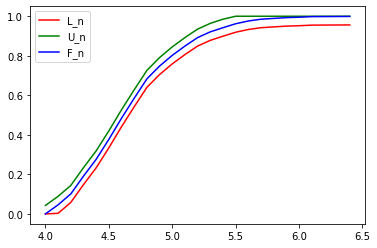
\includegraphics{Figure-08-03}
\end{figure}


\begin{python}
# Now to find the confidence interval, using the result from 8.5.6:
import math
from scipy.stats import norm
z_95 = norm.ppf(.975)
theta = F_n(4.9) - F_n(4.3)
se = math.sqrt(theta * (1 - theta) / n)
print('95%% confidence interval: (%.3f, %.3f)' % ((theta - z_95 * se), (theta + z_95 * se)))
\end{python}
\begin{console}
95\% confidence interval: (0.526, 0.588)
\end{console}

\textbf{Exercise 8.5.8}. Get the data on eruption times and waiting
times between eruptions of the old faithful geyser from the course
website.
\begin{itemize}[tightlist]
\item
  Estimate the mean waiting time and give a standard error for the
  estimate.
\item
  Also, give a 90\% confidence interval for the mean waiting time.
\item
  Now estimate the median waiting time.
\end{itemize}
In the next chapter we will see how to get the standard error for the
median.

\begin{python}
import numpy as np
import pandas as pd
data = pd.read_csv('data/geysers.csv', sep=',')
r = np.array(data['waiting'])
\end{python}

\begin{python}
# Estimate the mean waiting time and give a standard error for the estimate.
theta = r.mean()
se = np.std(r, ddof=1) / np.sqrt(len(r))
## Alternatively:
# from scipy.stats import sem
# se = sem(r)
print("Estimated mean: %.3f" % theta)
print("Estimated SE: %.3f" % se)
\end{python}
\begin{console}
Estimated mean: 70.897
Estimated SE: 0.824
\end{console}

\begin{python}
# Also, give a 90% confidence interval for the mean waiting time.
import math
from scipy.stats import norm
z_90 = norm.ppf(.95)
print('90%% confidence interval: (%.3f, %.3f)' % ((theta - z_90 * se), (theta + z_90 * se)))
\end{python}
\begin{console}
90\% confidence interval: (69.541, 72.253)
\end{console}

\begin{python}
# Now estimate the median time
median = np.median(r)
print("Estimated median time: %.3f" % median)
\end{python}
\begin{console}
Estimated median time: 76.000
\end{console}

\textbf{Exercise 8.5.9}. 100 people are given a standard antibiotic to
treat an infection and another 100 are given a new antibiotic. In the
first group, 90 people recover; in the second group, 85 people recover.
Let \(p_{1}\) be the probability of recovery under the standard treatment,
and let \(p_{2}\) be the probability of recovery under the new treatment.
We are interested in estimating \(\theta = p_{1} - p_{2}\). Provide an
estimate, standard error, an 80\% confidence interval and a 95\%
confidence interval for \(\theta\).

\textbf{Solution}. Let \(X_{1}, \dots, X_{1}00\) be indicator random
variables (0 or 1) determining recovery on the first group, and
\(Y_{1}, \dots, Y_{1}00\) indicating recovery on the second group. From the
problem formulation, we can assume \(X_{i} \sim \text{Bernoulli}(p_{1})\)
and \(Y_{i} \sim \text{Bernoulli}(p_{2})\). \(n_{1} = n_{2} = 100\), so we can
use \(n\) to refer to both.
If \(\theta = p_{1} - p_{2}\), then from exercise 8.5.2:
\[
\hat{\theta} = \hat{p}_{1} - \hat{p}_{2}
\]
\[
\SE (\hat{\theta}) = \sqrt{\frac{\hat{p}_{1}(1 - \hat{p}_{1})}{n} + \frac{\hat{p}_{2}(1 - \hat{p}_{2})}{n}}
\]

\begin{python}
import math
p_hat_1 = 0.9
p_hat_2 = 0.85
n = 100
theta_hat = p_hat_1 - p_hat_2
se_theta_hat = math.sqrt((p_hat_1 * (1 - p_hat_1) + p_hat_2 * (1 - p_hat_2)) / n)
print('Estimated mean: %.3f' % theta_hat)
print('Estimated SE: %.3f'   % se_theta_hat)
\end{python}
\begin{console}
Estimated mean: 0.050
Estimated SE: 0.047
\end{console}

\begin{python}
from scipy.stats import norm
z_80 = norm.ppf(.9)
z_95 = norm.ppf(.975)
print('80%% confidence interval: (%.3f, %.3f)' % ((theta_hat - z_80 * se_theta_hat), 
                                                 (theta_hat + z_80 * se_theta_hat)))
print('95%% confidence interval: (%.3f, %.3f)' % ((theta_hat - z_95 * se_theta_hat), 
                                                 (theta_hat + z_95 * se_theta_hat)))
\end{python}
\begin{console}
80\% confidence interval: (-0.010, 0.110)
95\% confidence interval: (-0.041, 0.141)
\end{console}

\textbf{Exercise 8.5.10}. In 1975, an experiment was conducted to see if
cloud seeding produced rainfall. 26 clouds were seeded with silver
nitrate and 26 were not. The decision to seed or not was made at random.
Get the data from the provided link.
Let \(\theta\) be the difference in the median precipitation from the
two groups.
\begin{itemize}[tightlist]
\item
  Estimate \(\theta\).
\item
  Estimate the standard error of the estimate and produce a 95\%
  confidence interval.
\end{itemize}

\begin{python}
import numpy as np
import pandas as pd
from tqdm import tqdm
data = pd.read_csv('data/cloud_seeding.csv', sep=',')
X = data['Seeded_Clouds']
Y = data['Unseeded_Clouds']
\end{python}

\begin{python}
theta_hat = X.median() - Y.median()
print('Estimated mean: %.3f' % theta_hat)
\end{python}
\begin{console}
Estimated mean: 177.400
\end{console}

\begin{python}
# Using bootstrap (from chapter 9):
nx = len(X)
ny = len(Y)
B = 10000
t_boot = np.zeros(B)
for i in tqdm(range(B)):
    xx = X.sample(n=nx, replace=True)
    yy = Y.sample(n=ny, replace=True)
    t_boot[i] = xx.median() - yy.median()
    
se = np.array(t_boot).std()
print('Estimated SE: %.3f' % se)
\end{python}
\begin{console}
100\%|███████████████████████████████████████████████████████████████████████████
████████████████████████████████████████████████████████████████████████████████
████████████████████████████████████| 10000/10000 [00:05<00:00, 1863.74it/s]
\end{console}
\begin{console}
Estimated SE: 63.420
\end{console}

\begin{python}
# See example 9.5, page 135
from scipy.stats import norm
z_95 = norm.ppf(.975)
normal_conf = (theta_hat - z_95 * se, theta_hat + z_95 * se)
percentile_conf = (np.quantile(t_boot, .025), np.quantile(t_boot, .975))
pivotal_conf = (2*theta_hat - np.quantile(t_boot, 0.975), 
                2*theta_hat - np.quantile(t_boot, .025))
print('95%% confidence interval (Normal): \t %.3f, %.3f' % normal_conf)
print('95%% confidence interval (percentile): \t %.3f, %.3f' % percentile_conf)
print('95%% confidence interval (pivotal): \t %.3f, %.3f' % pivotal_conf)
\end{python}
\begin{console}
95\% confidence interval (Normal):        53.099, 301.701
95\% confidence interval (percentile):    38.336, 266.201
95\% confidence interval (pivotal):       88.599, 316.464
\end{console}
